\section{Results}
Here, we set the parameters as default values and observe its performance. As the following figure shows, the energy always decreases or has some turning point and is always negative. Such as the red line, it has a peak due to a mismatch, and in our model, we find that it doesn't make the energy positive. It means that in this reaction process there is some force like "momentum" pushing it to proceed and cross the energy peak. Corresponding to the other figure's two particular locations (a and b), only in these points their energy are all negative (because we want to see the idea target series, only the locations which correspond to negative energy are collected).
\begin{figure}[h]
\centering
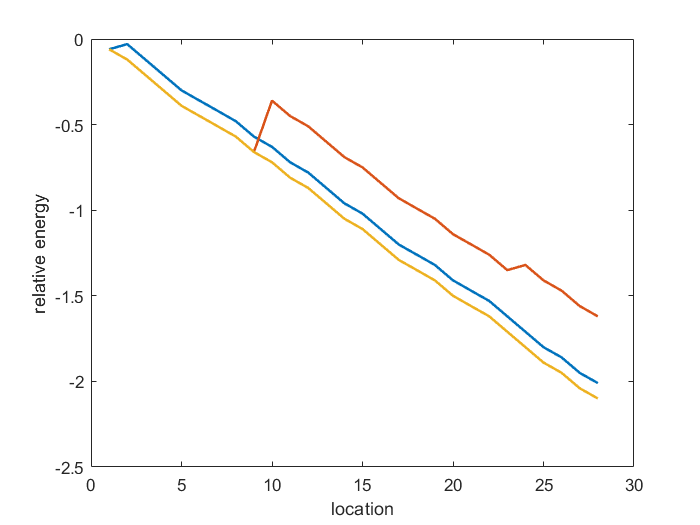
\includegraphics[width=0.7\linewidth]{energy_change}
\caption{energy change}
\label{fig:energychange}
\end{figure}

After testing our code run time, its manage rate can reach approximate $2\times10^8\;base/h$ (under parallel calculation in 4 cores) and have somewhat application value. 

\begin{figure}[h]
\centering
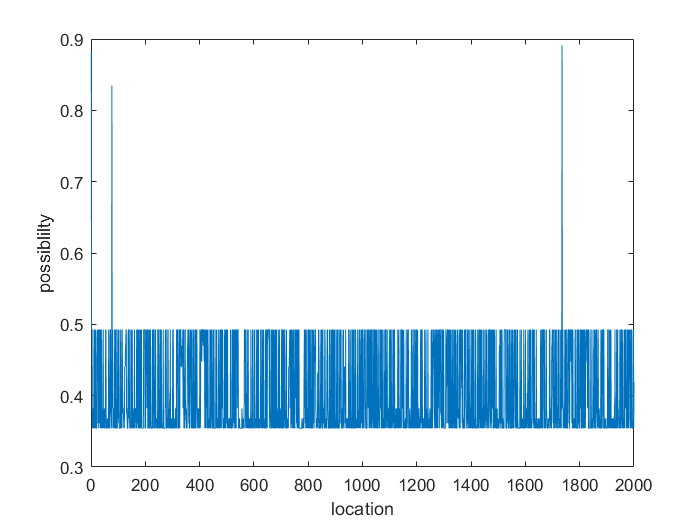
\includegraphics[width=0.7\linewidth]{fig1}
\caption{the possibility of target binding to nucleotide array in different location}
\label{}
\end{figure}

Besides the default parameters, we hope our model can hit more true data. So if we get the experiment data, we can use model 2.2 to get greater parameters. (@@no experiment data) 
